%% Auto-generated by scripts/generate_figures.py
\begin{figure}[htbp]
\centering
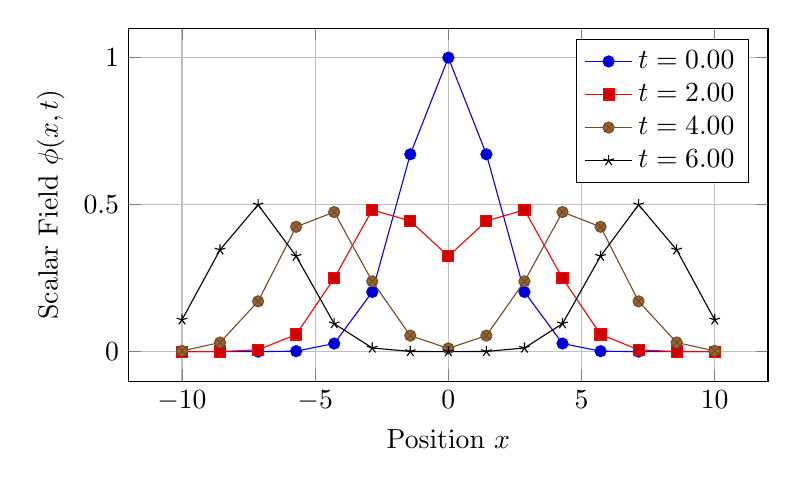
\begin{tikzpicture}
  \begin{axis}[
    width=0.8\textwidth,
    height=0.5\textwidth,
    xlabel={Position $x$},
    ylabel={Scalar Field $\phi(x,t)$},
    grid=major,
    legend pos=north east
  ]
    \addplot coordinates {
      (-10.0000, 3.293714e-09)
      (-8.5714, 5.863235e-07)
      (-7.1429, 4.701504e-05)
      (-5.7143, 1.699225e-03)
      (-4.2857, 2.767160e-02)
      (-2.8571, 2.030425e-01)
      (-1.4286, 6.712505e-01)
      (0.0000, 1.000000e+00)
      (1.4286, 6.712505e-01)
      (2.8571, 2.030425e-01)
      (4.2857, 2.767160e-02)
      (5.7143, 1.699225e-03)
      (7.1429, 4.701504e-05)
      (8.5714, 5.863235e-07)
      (10.0000, 3.293714e-09)
    };
    \addlegendentry{$t = 0.00$}
    \addplot coordinates {
      (-10.0000, 6.303553e-06)
      (-8.5714, 2.940227e-04)
      (-7.1429, 6.178252e-03)
      (-5.7143, 5.851035e-02)
      (-4.2857, 2.497416e-01)
      (-2.8571, 4.822695e-01)
      (-1.4286, 4.443937e-01)
      (0.0000, 3.246525e-01)
      (1.4286, 4.443937e-01)
      (2.8571, 4.822695e-01)
      (4.2857, 2.497416e-01)
      (5.7143, 5.851035e-02)
      (7.1429, 6.178252e-03)
      (8.5714, 2.940227e-04)
      (10.0000, 6.303553e-06)
    };
    \addlegendentry{$t = 2.00$}
    \addplot coordinates {
      (-10.0000, 2.543035e-03)
      (-8.5714, 3.108076e-02)
      (-7.1429, 1.711435e-01)
      (-5.7143, 4.246807e-01)
      (-4.2857, 4.748254e-01)
      (-2.8571, 2.392126e-01)
      (-1.4286, 5.456120e-02)
      (0.0000, 1.110900e-02)
      (1.4286, 5.456120e-02)
      (2.8571, 2.392126e-01)
      (4.2857, 4.748254e-01)
      (5.7143, 4.246807e-01)
      (7.1429, 1.711435e-01)
      (8.5714, 3.108076e-02)
      (10.0000, 2.543035e-03)
    };
    \addlegendentry{$t = 4.00$}
    \addplot coordinates {
      (-10.0000, 1.081326e-01)
      (-8.5714, 3.462900e-01)
      (-7.1429, 4.996817e-01)
      (-5.7143, 3.248924e-01)
      (-4.2857, 9.518200e-02)
      (-2.8571, 1.256433e-02)
      (-1.4286, 7.477073e-04)
      (0.0000, 4.006530e-05)
      (1.4286, 7.477073e-04)
      (2.8571, 1.256433e-02)
      (4.2857, 9.518200e-02)
      (5.7143, 3.248924e-01)
      (7.1429, 4.996817e-01)
      (8.5714, 3.462900e-01)
      (10.0000, 1.081326e-01)
    };
    \addlegendentry{$t = 6.00$}
  \end{axis}
\end{tikzpicture}
\caption{Temporal evolution of a Gaussian scalar field pulse propagating through vacuum.}
\label{fig:scalar-evolution}
\end{figure}
